\documentclass{beamer}

%\usetheme{Madrid}
%\usetheme{Boadilla}
%\usetheme{default}
%\usetheme{Warsaw}
%\usetheme{Bergen}
%\usetheme{Frankfurt}
\usetheme{Darmstadt}

\setbeamercolor{normal text}{fg=white}
\setbeamertemplate{background canvas}[vertical shading] [top=black!95,bottom=black!65]

\definecolor{mypurple}{RGB}{207,78,64}
\usecolortheme[named=mypurple]{structure}

\definecolor{myorange}{RGB}{255,235,190}
\beamerboxesdeclarecolorscheme{orange}{orange}{myorange}

\definecolor{commandcolor}{RGB}{111,195,165}

\setbeamertemplate{footline}[page number]
%\setbeamercovered{transparent}
\setbeamercovered{invisible}
\setbeamertemplate{navigation symbols}{}

%\usepackage{musixtex}
\usepackage{multimedia}
\usepackage{graphicx}
\usepackage[utf8]{inputenc}
%\usepackage[T1]{fontenc}
\usepackage[french]{babel} 
%\usepackage[all]{xy}
%\usepackage{multirow}
%\usepackage{lmodern}
\usepackage{subfigure}
%\usepackage{ulem}
\usepackage{url}
\usepackage{hyperref}
\usepackage{verbatim}
\usepackage{xspace}
\usepackage{color}
\usepackage{xcolor}
\usepackage{rotating}
\usepackage{multicol}
\usepackage[export]{adjustbox}
\usepackage{textpos}
\usepackage{listings}
\usepackage{fontawesome}


\definecolor{mypurple}{RGB}{207,78,64}
\usecolortheme[named=mypurple]{structure}

\definecolor{myorange}{RGB}{255,235,190}
\beamerboxesdeclarecolorscheme{orange}{orange}{myorange}

\definecolor{dgreen}{RGB}{0,125,0}

\usepackage{tikz}
\usetikzlibrary{trees}

\setbeamertemplate{caption}[numbered] 

\newcommand{\setframetitle}[1]{\begin{center}
    \huge \textbf{#1}
\end{center}}


\lstset{
    %frame=tb, % draw a frame at the top and bottom of the code block
    tabsize=4, % tab space width
    showstringspaces=false, % don't mark spaces in strings
    numbers=left, % display line numbers on the left
    commentstyle=\color{green}, % comment color
    keywordstyle=\color{myorange}, % keyword color
    stringstyle=\color{mypurple} % string color
}

%% --------------

\title{Gnuplot}
\subtitle{Atelier d'aide à la programmation}
\author{L\'eo \textsc{Baudouin}}
\institute{
  {\url{baudouin.leo @ gmail.com}}
}
\date{03-04 juin 2019}

%% --------------

\begin{document}

\begin{frame}
  \titlepage
\end{frame}

\section{Introduction}
\subsection{}

\begin{frame}{Exemple d'utilisation}
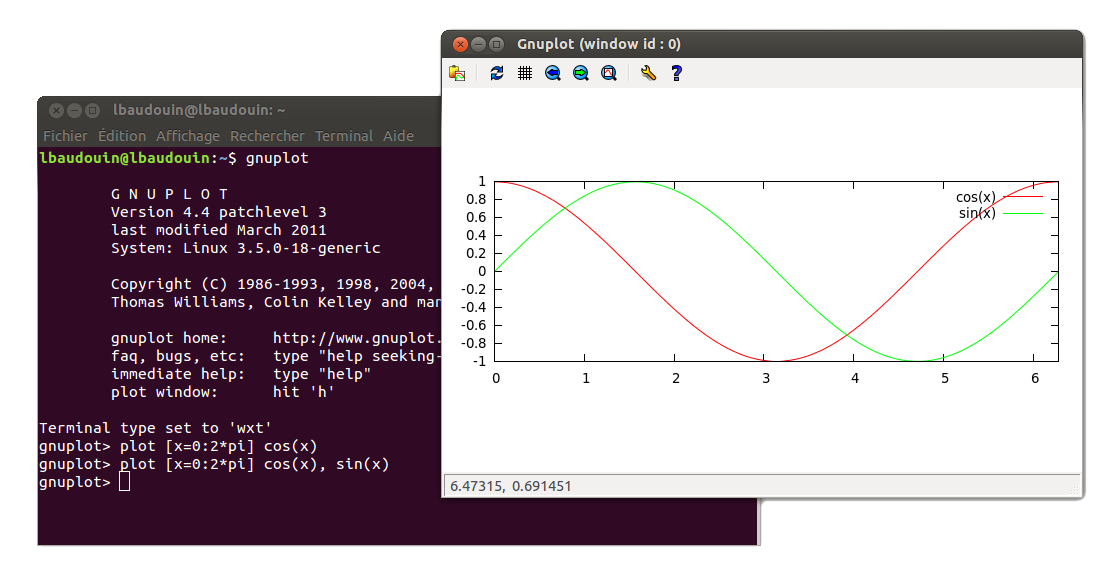
\includegraphics[width=\linewidth]{images/gnuplot-exemple}

\begin{center}
\verb?plot [x=0:2*pi] cos(x), sin(x)?
\end{center}
\end{frame}

\begin{frame}
\begin{scriptsize}
\begin{tabular}{c l}
Space      &   raise gnuplot console window \\
 q         &    quit X11 terminal \\
 a         &    `builtin-autoscale` (set autoscale keepfix; replot) \\
 b         &    `builtin-toggle-border` \\
 e         &    `builtin-replot` \\
 g         &    `builtin-toggle-grid` \\
 h         &    `builtin-help` \\
 l         &    `builtin-toggle-log` y logscale for plots, z and cb logscale for splots \\
 L         &    `builtin-nearest-log` toggle logscale of axis nearest cursor \\
 m         &    `builtin-toggle-mouse` \\
 r         &    `builtin-toggle-ruler` \\
 1         &    `builtin-decrement-mousemode` \\
 2         &    `builtin-increment-mousemode` \\
 3         &    `builtin-decrement-clipboardmode` \\
 4         &    `builtin-increment-clipboardmode` \\
 5         &    `builtin-toggle-polardistance` \\
 6         &    `builtin-toggle-verbose` \\
 7         &    `builtin-toggle-ratio` \\
 n         &    `builtin-zoom-next` go to next zoom in the zoom stack \\
 p         &    `builtin-zoom-previous` go to previous zoom in the zoom stack \\
 u         &    `builtin-unzoom` \\
 Right     &    `builtin-rotate-right` only for splots; \textless shift\textgreater{} increases amount \\
 Up        &    `builtin-rotate-up` only for splots; \textless shift\textgreater{} increases amount \\
 Left      &    `builtin-rotate-left` only for splots; \textless shift\textgreater{} increases amount \\
 Down      &    `builtin-rotate-down` only for splots; \textless shift\textgreater{} increases amount \\
 Escape    &    `builtin-cancel-zoom` cancel zoom region
\end{tabular}
\end{scriptsize}
\end{frame}

\section{Plot et splot}
\subsection{}
\begin{frame}[fragile]{Plot}

\begin{block}{Cloner le dép\^ot suivant}
\url{https://github.com/lbaudouin/module-gnuplot.git}
\end{block}

\begin{block}{Tracer des données}
\verb?pop(x)=103*exp((1965-x)/10)?\linebreak
\verb?plot [1960:1990] 'population.dat', pop(x)?
\end{block}

\begin{block}{Définir les commentaires dans un fichier}
\verb?set datafile commentschars "#%"?\linebreak
Pour l'ajouter de façon permanente, le mettre dans le fichier : \verb?~/.gnuplot?
\end{block}
\end{frame}

\begin{frame}{Titres}

\begin{block}{Modifier les titres}
\begin{itemize}
\item Modifier le titre de la courbe :\\
\verb?plot pop(x) title "Nouveau titre"?\\
\verb?plot pop(x) t "Nouveau titre"?
\item Ajouter un titre au graphique :\\ \verb?set title "Titre du graphique"?
\end{itemize}
\end{block}
\end{frame}

\begin{frame}{Styles}

\begin{block}{Plot}
\verb?plot sin(x) with <style>?\\
\verb?plot sin(x) w <style>?
\end{block}

\begin{block}{Styles de courbe}
\begin{tabular}{l l l}
\textbf{nom} & \textbf{raccourci} & \textbf{description} \\
\hline
boxes   &   & rectangles verticaux \\
dots    & d & petits points \\
errorbars & e & points et barre verticale d'erreur \\
impulses  & i & lignes verticales \\
lines     & l &       lignes\\
linespoints & lp &   lignes et points\\
points      & p &     points\\
steps      & st &      marche d'escalier
\end{tabular}
\end{block}
\end{frame}

\begin{frame}{Couleurs}

\begin{block}{Ajouter des couleurs}
\verb?plot sin(x) linecolor 1?\\
\verb?plot sin(x) lc 3?
\end{block}

\begin{block}{Correspondance des couleurs}
\begin{tabular}{c l | c l}
1 & red & 6 & yellow \\
2 & green & 7 & black \\
3 & 	blue & 8 & orange \\ 
4 & 	magenta & 9 & grey \\
5 &	lightblue
\end{tabular}

\end{block}

\end{frame}


\begin{frame}{Colonnes d'un fichier}

\begin{block}{Utilisation des colonnes}
\verb?splot "pts3D.txt" using 1:3:2?\\
\verb?splot "pts3D.txt" u 1:3:(-\$2)?
\end{block}

\begin{block}{Combiner couleurs et colonnes}
\verb?plot "path.txt" u 1:2:0 w lp lc palette?
\end{block}

\end{frame}


\section{Génération d'image}
\subsection{Version 1}
\begin{frame}[fragile]{Utiliser Gnuplot dans vos programmes}
\begin{block}{Commande}
\verb?system("gnuplot file.gnup")?
\end{block}

\begin{block}{file.gnup}
  \begin{lstlisting}[language=C++]
set term png size 1024,768
set out "output.png"
set xr [-10:2]
set yr [-2:10]
unset label
set view equal xyz
splot 'x.txt' w l, 'y.txt' w l, 'z.txt' w l
\end{lstlisting}
\end{block}
\end{frame}

\section{Génération d'image}
\subsection{}
\subsection{Version 2}
\begin{frame}[fragile]{Utiliser Gnuplot dans vos programmes}
\begin{block}{Installer une API}
\verb?sudo apt install libgnuplot-iostream-dev?
\end{block}

\begin{block}{\url{http://stahlke.org/dan/gnuplot-iostream/}}
\tiny
  \begin{lstlisting}[language=C++]
#include <map>
#include <vector>
#include <cmath>
#include "gnuplot-iostream.h"
int main() {
	Gnuplot gp;
	std::vector<std::pair<double, double> > xy_pts_A;
	for(double x=-2; x<2; x+=0.01) {
		xy_pts_A.push_back(std::make_pair(x, x*x*x));
	}
	std::vector<std::pair<double, double> > xy_pts_B;
	for(double alpha=0; alpha<1; alpha+=1.0/24.0) {
		double theta = alpha*2.0*3.14159;
		xy_pts_B.push_back(std::make_pair(cos(theta), sin(theta)));
	}
	gp << "set xrange [-2:2]\nset yrange [-2:2]\n";
	gp << "plot" << gp.file1d(xy_pts_A) << "with lines title 'cubic',"
	   << gp.file1d(xy_pts_B) << "with points title 'circle'" << std::endl;
}
\end{lstlisting}
\end{block}
\end{frame}


%-------------------------------------------------------------------

\end{document} 

%-------------------------------------------------------------------

%\transdissolve[duration=0.25]
%
%\begin{exampleblock}{Avantages}
%\end{exampleblock}
%
%\begin{alertblock}{Inconvénients}
%\end{alertblock}
